\chapter{Verwandte Arbeiten}
\label{sec:relatedwork}

Dieses Kapitel ordnet die vorliegende Methodik in den aktuellen wissenschaftlichen Diskurs ein. Dabei werden etablierte Verfahren der Container-Analyse kritisch bewertet und bestehende methodische Lücken im Kontext der Feature-Extraktion (TF1) sowie der Zuordnung zu spezifischen Erzeugerquellen (TF2) aufgezeigt.

Während die klassische Multimedia-Forensik zur Quellenerkennung, insbesondere sensorbasierte Ansätze wie PRNU, ein reifes Forschungsfeld darstellt \cite{lukas_digital_2006}, ist die Nutzung der reinen Metadaten-Grammatik zur Generierung kompakter Dateisignaturen ein neuerer methodischer Ansatz von \citeauthor{klier_media_2025} \cite{klier_media_2025}. Auch das wertbasierte Approximate Matching auf Byte-Ebene ist zur Erkennung binärer Dateiähnlichkeiten in der Forensik seit Längerem etabliert \cite{roussev_data_2010}. Die Schnittmenge dieser beiden Domänen, also das syntaktische Similarity Hashing von Mediencontainern zur Identifikation von Erzeugerquellen, bildet hingegen eine aktuelle methodische Entwicklung ab.

\section{Container-basierte Video-Forensik}

Die etablierte Videoforensik stützt sich primär auf die Analyse des audiovisuellen Bitstroms, was durch die Notwendigkeit der vollständigen Dekodierung rechenintensiv ist und durch verlustbehaftete Kompressionsprozesse erschwert wird \cite[Kap. 1]{yang_comprehensive_2025}. Als effiziente Alternative hat sich die isolierte Auswertung von Datei-Containern etabliert, welche die medienspezifischen Streams umgeht und ausschließlich die syntaktischen Metadatenstrukturen untersucht \cite[Kap. 3]{yang_comprehensive_2025}. Die anhaltende Relevanz dieses Forschungsfeldes belegen die aktuellen Untersuchungen von Yang u.,a. (2025) \cite{yang_comprehensive_2025}.

\begin{figure}[h]
    \centering
    
\includegraphics[width=1\linewidth]{yang.drawio.png}
    \caption{TODO: yang.drawio.png}
    \label{fig:yang}
\end{figure}

Yang u.\,a. (2025) ordnen die primären forensischen Aufgabenbereiche der Container-Analyse in vier Kategorien (siehe \cref{fig:yang}) ein \cite{yang_comprehensive_2025}. Der erste Bereich umfasst die Identifikation der Quellkamera (\textit{Source Camera Identification}, SCI), um eine Datei einer spezifischen Hardwarekomponente oder Marke zuzuordnen \cite[Kap. 5.4.6]{yang_comprehensive_2025}. Die Identifikation der Manipulationssoftware (\textit{Manipulation Tool Identification}, MTI) fokussiert sich auf den Nachweis spezifischer Bearbeitungsprogramme \cite[Kap. 5.4.5]{yang_comprehensive_2025}. Die Erkennung plattformspezifischer Signaturen durch den Upload auf soziale Netzwerke wird durch die Zuordnung zu sozialen Netzwerken (\textit{Social Network Attribution}, SNA) adressiert \cite[Kap. 5.4.4]{yang_comprehensive_2025}. Schließlich bildet die Manipulationserkennung (\textit{Video Manipulation Detection}, MD) den Bereich ab, der strukturelle Anomalien aufdeckt, die durch die syntaktische Neukapselung des Containers bei der Bearbeitung entstehen \cite[Kap. 5.4.7]{yang_comprehensive_2025}.\\

%%%

\subsection{Grundlagen der isolierten Container-Auswertung und Taxonomie}

TODO: Ggf. nochmal auf 2 Kapitel aufteilen\\

Die wissenschaftliche Fundierung dieser Methodik wurde maßgeblich durch die richtungsweisende Arbeit von Gloe u.\,a. (2014) gelegt \cite{gloe_forensic_2014}. Das zentrale Ergebnis ihrer Untersuchung wies nach, dass Dateiformat-Standards den herstellenden Unternehmen sowie entwickelnden Personen erhebliche Freiheitsgrade bei der konkreten softwareseitigen Implementierung einräumen \cite[S. S68]{gloe_forensic_2014}. Konkret zeigten Gloe u.\,a., dass Spezifikationen wie das ISOBMFF zwar grundlegende syntaktische Regeln definieren, die exakte Reihenfolge optionaler Boxen, die Strukturierung von Metadaten-Blöcken sowie das Einfügen proprietärer Erweiterungen jedoch optional belassen \cite[S. S68]{gloe_forensic_2014}. Im Ergebnis dokumentierte die Arbeit, dass diese systemspezifischen Designentscheidungen zu signifikanten und messbaren syntaktischen Abweichungen zwischen verschiedenen Kamera- und Software-Systemen führen \cite[S. S69]{gloe_forensic_2014}.

Hinsichtlich der konkret genutzten Formate und Codecs belegt die Studie von Gloe u.\,a. (2014) diese herstellerspezifische Spurbildung anhand eines eigens für diese Untersuchung aufgebauten Datensatzes sowie deutlicher technischer Unterschiede zwischen den Geräteklassen \cite{gloe_forensic_2014}. Die Ergebnisse zeigen, dass Mobiltelefone primär MP4-ähnliche Container nutzen und komplexe Kompressionsalgorithmen wie MP4V oder die H.26x-Familie verwenden. Wie in Tabelle \ref{tab:gloe} exemplarisch dargestellt, führt diese herstellerspezifische Implementierung bereits bei der Auswahl und Platzierung optionaler Struktur-Boxen zu charakteristischen Signaturen. So nutzen einige Smartphones die optionalen Boxen \(free\) oder \(meta\) und andere positionieren die \(mdat\)-Box erst ans Ende der Baumstruktur. Diese Abweichungen in der Standardkonfiguration der Dateisysteme bekräftigen die Annahme, dass die rein syntaktische Zusammensetzung des Dateiformats konkrete Rückschlüsse auf die Geräteklasse der Erzeugerquelle zulässt.

\begin{table}[htbp]
    \centering
    \begin{tabular}{>{\raggedright\arraybackslash}p{0.5\linewidth}>{\raggedright\arraybackslash}p{0.44\linewidth}}\hline\hline
         \textbf{Smartphones}& \textbf{Optionale Boxen}\\\hline\hline
         BlackBerry 8310, Google Nexus 7, Motorola MileStone, Palm Pre, Samsung GT-5500i, SonyEricsson K800i& \(udta\)\\\hline
         iPhone 4& \(wide, free, meta\)\\\hline
         Benq S88& \(mvex, moof, mdat\) (am Dateiende)\\\hline
         Nokia X3-00 & \(free, mdat\) (am Dateiende)\\\hline
         Samsung SGH-D600& \(iods\)\\ \hline\hline
    \end{tabular}
    \caption{Signifikante strukturelle Abweichungen in der Verwendung optionaler MP4-Atome bereits in 2014 (Eigene Darstellung nach Gloe u. a. \cite[Tab. 4]{gloe_forensic_2014})}
    \label{tab:gloe}
\end{table}

Die fortdauernde Relevanz dieser Grundlagen wird durch die Ergebnisse der systematischen Übersichtsarbeit von Yang u.\,a. (2025) untermauert und in den aktuellen Stand der Technik überführt \cite{yang_comprehensive_2025}. Als primäres Ergebnis weisen sie nach, dass die isolierte Container-Analyse im Vergleich zu rechenintensiven, pixelbasierten Deep-Learning-Verfahren eine drastisch reduzierte algorithmische Komplexität aufweist und so eine performante Analyse von großen Datenmengen ermöglicht \cite[Kap. 4]{yang_comprehensive_2025}. Ein weiteres zentrales Resultat ihrer Arbeit ist der Nachweis, dass die verwendeten Manipulations- und Bearbeitungswerkzeuge bei der Neukapselung fast ausnahmslos charakteristische, anomale Spuren in der Container-Grammatik hinterlassen \cite[Kap. 5]{yang_comprehensive_2025}. Die Ergebnisse von Yang u.\,a. (2025) bestätigen damit, dass die syntaktische Strukturprüfung von MP4-Dateien ein hochwirksames Instrument zur forensischen Zuordnung und Identifikation der Erzeugersoftware darstellt.

Zur Strukturierung dieses Forschungsfeldes schlagen Yang u.\,a. (2025) eine Taxonomie vor, welche die existierenden containerbasierten Forensikverfahren in eine qualitative und eine quantitative Analyse kategorisiert \cite{yang_comprehensive_2025}. Während die qualitative Analyse auf dem direkten Vergleich von Containerstrukturen basiert, umfasst die quantitative Analyse eine mehrstufige Pipeline aus Parsing, symbolischer Repräsentation, Merkmalsselektion, Merkmalsdarstellung und Klassifikation \cite[Kap. 4]{yang_comprehensive_2025}.

\begin{table}
    \centering
    \begin{tabular}{>{\raggedright\arraybackslash}p{0.05\linewidth}>{\raggedright\arraybackslash}p{0.12\linewidth}>{\raggedright\arraybackslash}p{0.31\linewidth}>{\raggedright\arraybackslash}p{0.4\linewidth}}\hline\hline
         \textbf{Typ}&  \textbf{Kategorie}&  \textbf{Eigenschaften}& \textbf{Vor- und Nachteile}\\\hline\hline
         T1&  Geordnet& 
         Komplette Ebenen-Info und strenge sequenzielle Nummerierung&+ Exakte Index-Erfassung\newline
- Sehr anfällig für Einfügen/Löschen\\\hline
         T2&  Geordnet&  Nur pfadrelevante Infos sequenzielle Nummerierung&+ Kompakter als T1\newline
- Anfällig für Einfügen/Löschen\\\hline
         T3&  Geordnet&  Nur pfadrelevante Infos und nummeriert nur gleichen Box-Typ&+ Robust bei allgemeinen Änderungen\newline
- Anfällig bei identischen Boxen davor\\\hline
         T4&  Ungeordnet&  Nur pfadrelevante Infos und ignoriert Reihenfolge komplett&+ Robust bei abweichenden Boxen\newline
- Anfällig bei identischen Boxen\\\hline
         T5&  Ungeordnet&  Nur finales Feld sowie Wert und verwirft Struktur-Pfad komplett& - Vollständiger Verlust der Struktur-Infos\\ \hline\hline
    \end{tabular}
    \caption{Repräsentationsmodelle für Video-Container (Eigene Darstellung nach Yang u.\,a. \cite[Tab. 2]{yang_comprehensive_2025}}
    \label{tab:yang}
\end{table}

Auf der Ebene der symbolischen Repräsentation wird der hierarchische MP4-Baum in maschinenlesbare Symbole überführt. Yang u.\,a. (2025) systematisieren die bisherigen Forschungsansätze hierbei in fünf Modelle (T1 bis T5), die sich grundlegend in geordnete und ungeordnete Darstellungsformen unterteilen lassen (siehe \cref{tab:yang}) \cite[Kap. 4.3.2]{yang_comprehensive_2025}. Geordnete Repräsentationen (T1, T2 und T3) speichern die strukturellen Pfade und nummerieren die Boxen sequenziell durch. Während T1 alle vorausgehenden Boxen strikt erfasst und somit extrem anfällig für strukturelle Veränderungen ist, reduzieren T2 und T3 die Pfadinformationen auf die unmittelbar relevanten Zielboxen. Dies erhöht die Robustheit gegenüber dem Einfügen oder Löschen von Boxen drastisch. Ungeordnete Repräsentationen (T4 und T5) ignorieren die sequenzielle Reihenfolge teilweise oder vollständig. T4 bewahrt die Pfadinformationen ohne deren Ordnung, was eine hohe Resilienz gegenüber der Modifikation abweichender Boxen bietet. T5 hingegen isoliert lediglich die reinen Feldwerte ohne jeglichen Strukturpfad, was zu einem vollständigen Verlust der topologischen Metadaten führt \cite[Kap. 4.3.2]{yang_comprehensive_2025}. Die Auswertungen von Yang u.\,a. belegen, dass die Repräsentationen T2, T3 und T4 die beste forensische Erkennungsleistung aufweisen, da sie eine optimale Balance zwischen struktureller Präzision und Robustheit bieten \cite[Kap. 5]{yang_comprehensive_2025}.

Im Schritt der \textit{Feature Representation} differenziert die Studie zwischen \textit{Bag-of-Words}- und \textit{Type-aware}-Modellen \cite[Kap. 4.3.4]{yang_comprehensive_2025}. Während Bag-of-Words absolute Häufigkeiten von Container-Symbolen zählt, übernimmt der Type-aware-Ansatz kontinuierliche Werte direkt numerisch, um die Dimensionalität des Feature-Vektors zu reduzieren. Die Ergebnisse belegen, dass die syntaktische Strukturprüfung ein hochwirksames Instrument zur Identifikation von Erzeugersoftware ist \cite{yang_comprehensive_2025}. 

Die Differenzierung dieser Repräsentationsmodelle verdeutlicht das methodische Bestreben, forensische Tiefe und algorithmische Effizienz bei der Verarbeitung hierarchischer Containerdaten bestmöglich zu vereinen und dient als Grundlage für das nachfolgende Kapitel \ref{sec:quant}.\\

TODO: Kurz-Erklärung für BOW und Type-aware nochmal verständlicher überarbeiten bzw. kürzen

%%%%


% hier noch alles korrigieren


\subsection{Quantitative Merkmalserfassung}
\label{sec:quant}

Innerhalb der quantitativen Container-Forensik dient die Merkmalsdarstellung dem Ziel, die aus der hierarchischen MP4-Struktur extrahierten Symbole in maschinenlesbare Vektoren zu übersetzen. Ein etabliertes Modell hierfür ist der \textit{Bag-of-Words}-Ansatz. Dieser behandelt die zuvor abgeleiteten Container-Symbole konzeptionell analog zu Vokabeln in der Textverarbeitung, indem er ausschließlich deren absolute Häufigkeit innerhalb der Datei zählt und in einem Feature-Vektor abbildet. Sofern die zugrunde liegende symbolische Repräsentation (wie bei den Modellen T1 bis T4) Pfadinformationen einschließt, bleibt die hierarchische Einbettung der Atome im Vektor erhalten.

Einen repräsentativen Ansatz für diese Methodik präsentierten Yang u.\,a. (2020). Sie entwickelten eine vektorielle Repräsentation der Containerstruktur, die sich an Bag-of-Words anlehnt, und nutzten Entscheidungsbäume, um die Integrität von Videodateien zu überprüfen sowie die verwendete Manipulationssoftware zu identifizieren \cite{yang_efficient_2020}. Xiang u.\,a. (2021) erweiterten dieses Konzept später zum \textit{Type-aware}-Ansatz, um neben der bloßen Zählung diskreter Boxen auch kontinuierliche Werte effizienter in den Vektoren zu verarbeiten \cite{xiang_forensic_2021}.

Die forensische Stärke von Bag-of-Words-Modellen und der generellen quantitativen Pipeline liegt in ihrer enormen algorithmischen Effizienz. Da sie auf dem Zählen von Frequenzen basieren und beim Vergleich von Dateien keine rechenintensiven, rekursiven Graphenabgleiche durchführen müssen, eignen sie sich exzellent für hochskalierbare Cloud-Umgebungen und Triage-Systeme. Ein methodischer Nachteil bezüglich des topologischen Kontextes entsteht lediglich dann, wenn als Vorstufe eine ungeordnete symbolische Repräsentation wie T5 gewählt wird. Bei T5 wird die Information über die exakte Pfadtiefe und die Eltern-Kind-Beziehung der Boxen vollständig verworfen und ausschließlich die Häufigkeit finaler Feldwerte gezählt, was die Unterscheidung stark ähnlicher Containerstrukturen signifikant erschwert \cite{yang_comprehensive_2025}.

%%%

\subsection{Qualitative und pfadbasierte Strukturanalyse}

Um den Verlust topologischer Informationen zu vermeiden, nutzt ein weiterer methodischer Strang den MP4-Container als strukturierten Baum und wertet die exakten Pfade und Eltern-Kind-Beziehungen der ISO-Boxen aus.

Ein grundlegendes Framework für diesen Ansatz legten Iuliani u.\,a. (2019) vor, die ein auf \textit{Likelihood-Ratios} basierendes quantitatives Modell zur unüberwachten Quellengeräte-Erkennung (SCI) entwickelten \cite{iuliani_video_2019}. Ihr Algorithmus analysiert die baumartige Metadaten-Architektur und berechnet die Wahrscheinlichkeit, mit der eine gegebene Container-Grammatik von einer spezifischen Smartphone-Marke erzeugt wurde. Dieser strukturbasierte Ansatz ermöglicht eine trennscharfe Zuordnung, da er die proprietären Designentscheidungen der Hersteller in ihrer syntaktischen Tiefe erfasst. Eine alternative Auswertung dieser topologischen Daten demonstrierten Ramos-López u.\,a. (2020) \cite{ramos_lopez_digital_2020}. Sie nutzen extrahierte Pfad- und Reihenfolge-Merkmale der Metadaten-Knoten, um digitale Videos mittels unüberwachter Clustering-Algorithmen (wie dem hierarchischen Clustering) auch ohne vorheriges Training spezifischen Quellgeräten zuzuordnen.

Die Limitierung streng geordneter Strukturauswertungen (vergleichbar mit den Repräsentationen T1 und T2 nach der Taxonomie von Yang u.\,a. \cite{yang_comprehensive_2025}) liegt in ihrer Inflexibilität. Der strikte Abgleich sequenzieller Pfade scheitert häufig in der Praxis, da bereits triviale, von der Software initiierte Einfügungen oder Verschiebungen optionaler Atome (wie \textit{free} oder \textit{udta}) die nachfolgenden Indizes verschieben. Dies verursacht eine signifikante Veränderung der abgebildeten Container-Reihenfolge, was den direkten forensischen Strukturvergleich erschwert.

%%%

\subsection{Limitationen bestehender Verfahren}

Die systematische Betrachtung der etablierten Analyseverfahren offenbart methodische Herausforderungen bei der Modellierung der Containerstruktur. Bisherige Ansätze zwingen die Forensik bei der symbolischen Repräsentation in ein Dilemma: Streng geordnete Modelle (wie T1 und T2) erfassen die Topologie präzise, reagieren aber auf minimale strukturelle Varianzen oder eingefügte Boxen äußerst fehleranfällig. Ungeordnete Modelle (insbesondere T5) skalieren durch ihre Abstraktion zwar hervorragend, verwerfen den hierarchischen Kontext der Metadaten jedoch vollständig \cite{yang_comprehensive_2025}.

Darüber hinaus weisen containerbasierte Ansätze eine grundlegende Schwachstelle auf: die Anfälligkeit gegenüber trivialem \textit{Re-Muxing} (Stream Copy) \cite{li_learning_2024}. Li u.\,a. (2024) kritisieren, dass die native, herstellerspezifische Container-Struktur durch einen einfachen Kopiervorgang mittels gängiger Software-Encoder überschrieben und durch die Signatur der Software ersetzt werden kann, ohne dass eine rechenintensive Transcodierung des audiovisuellen Bitstroms erfolgt \cite{li_learning_2024}. Für maschinelle Klassifikatoren, die auf starre Container-Strukturen trainiert wurden, geht der ursprüngliche forensische Fingerabdruck des Aufnahmegeräts dadurch verloren, was die Bestimmung der Originalquelle drastisch erschwert.

Diese Limitationen verdeutlichen die Notwendigkeit eines flexiblen und fehlertoleranten Analyseverfahrens auf syntaktischer Ebene. Die Transformation der hierarchischen Metadatenstrukturen in sequenzielle Token, gepaart mit einem \textit{Similarity Hashing} -- dem methodischen Kern dieser Arbeit --, bietet das Potenzial, die Skalierbarkeit quantitativer Verfahren zu wahren und den kontextuellen Pfadverlust zu verhindern \cite{klier_media_2025}. Gleichzeitig soll dadurch eine höhere algorithmische Resilienz gegenüber standardkonformen Strukturverschiebungen erzielt werden.
\section{Similarity Hashing in der Multimedien-Forensik}
\label{sec:similarity_hashing_multimedia}

Einen grundlegenden Beitrag in diesem Bereich lieferten Klier und Baier mit dem Framework des Media Source Similarity Hashing (MSSH), welches als das erste rein syntaktische Approximate-Matching-Verfahren zur Quellenerkennung eingeführt wurde \cite[Kap. 1]{klier_media_2025}. MSSH extrahiert die Sequenz der Format-Marker von JPEG-Dateien, überführt diese mittels n-Gramm-Sequenzierung in ein Token-Set und komprimiert das Ergebnis zu einem effizient vergleichbaren Similarity Digest (siehe \cref{fig:vorgeh-mssh}) \cite[Kap. 3]{klier_media_2025}.

\begin{table}
    \centering
    \begin{tabular}{>{\raggedright\arraybackslash}p{0.2\linewidth}>{\raggedright\arraybackslash}p{0.75\linewidth}}\toprule
         \textbf{Studie}& Klier und Baier (2025)\cite{klier_media_2025}\\\midrule
         \textbf{Verfahren}& MSSH (Media Source Similarity Hashing)\\\midrule
         \textbf{Untersuchungsziele}& SCI (Source Camera Identification auf Geräte-, Modell- und Markenebene, z. B. zur Unterscheidung von Downloads und Eigenproduktionen in CSAM-Ermittlungen) und SNA (Erkennung der Verarbeitung durch 5 Social-Media-Plattformen)\\\midrule
         \textbf{Feature}& Strukturelle Marker und deren Reihenfolge (z. B. das 2-Gramm D8E1 aus den aneinandergereihten JPEG-Markern SOI und APP1)\\\midrule
         \textbf{Symbolische Repräsentation} (T1 bis T5)& TODO\\\midrule
         \textbf{Feature-Repräsentation}& n-Gramm-Sets (Similarity Digest)\\\midrule
         \textbf{Feature-Selektion}& Dubletteneliminierung (reduziert die Sequenzen auf eine rein binäre Mengen-Repräsentation, Worthäufigkeiten werden ignoriert)\\\midrule
         \textbf{Klassifikator}& Approximate Matching (Ähnlichkeitsberechnung mittels Jaccard-Index oder asymmetrischem Tversky-Index)\\\midrule
         \textbf{Datenbanken}& 7 Bilddatensätze (u. A. VISION)\\\midrule
         \textbf{Test- und Trainingsdaten}& Bildung von Referenz-Hashes (Source Similarity Digests) aus einer kleinen, diversen Teilmenge (z. B. ein Bild pro Aufnahmemodus), Abgleich mit allen restlichen Testdateien\\\midrule
         \textbf{Evaluation}&Klassifikation auf Geräte-, Modell- und Markenebene sowie Erkennung der Verarbeitung durch 5 Social-Media-Plattformen\\\midrule
         \textbf{Metriken}&Receiver Operating Characteristic (ROC) und Area Under Curve (AUC)\\ \bottomrule
    \end{tabular}
    \caption{Verfahrenssteckbrief zum Media Source Similarity Hashing (Eigene Darstellung nach Klier und Baier\cite{klier_media_2025} }
    \label{tab:steckbrief-klier}
\end{table}

\begin{figure}
    \centering
    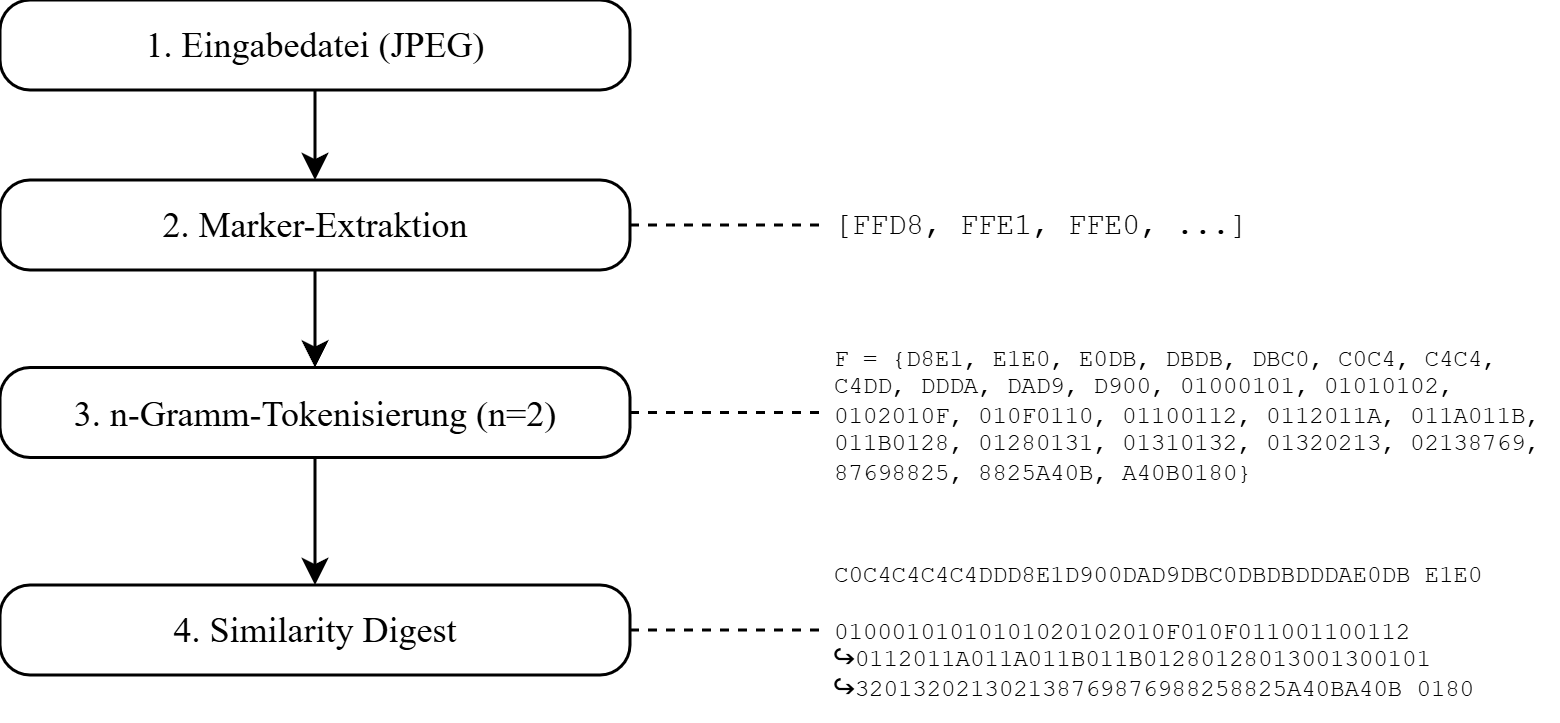
\includegraphics[width=0.9\linewidth]{grafiken/vorgehen-mssh.drawio.png}
    \caption{TODO: vorgehen-mssh.drawio.png}
    \label{fig:vorgeh-mssh}
\end{figure}

Das Konzept des $n$-Gramms stammt ursprünglich aus der Computerlinguistik und bezeichnet eine Abfolge von $n$ aufeinanderfolgenden Elementen in einer Datenreihe \cite[Kap. 3]{jurafsky_speech_2026}. Wendet man dies auf Dateistrukturen an, wandert ein festes Sichtfenster (Sliding Window) der Länge $n$ schrittweise über die extrahierten Format-Marker. So entsteht eine Menge an überlappenden Teilsequenzen. Der Vorteil dieser Methode ist, dass lokale Bausteine und ihre Reihenfolge erhalten bleiben. Dadurch lassen sich Dateien auch dann zuverlässig vergleichen, wenn sie nicht vollständig, sondern nur in bestimmten Teilbereichen strukturell übereinstimmen \cite[Kap. 3.2]{klier_media_2025}.

Die exakte Reihenfolge und das Auftauchen struktureller Elemente besitzen für die forensische Differenzierung von Quellen eine hohe Prägnanz. Bei der Übertragung dieses Prinzips auf Videodaten ergeben sich neue Herausforderungen. Wie in Abschnitt \ref{kap:aufbau_mp4} dargelegt, basiert die Architektur von MP4-Dateien nicht auf einer linearen Abfolge von Markern, sondern auf einer tief verschachtelten, objektorientierten Baumstruktur \cite[Kap. 4]{iso_14496-12_2022}.

Die grundlegende Methodik des MSSH weist mehrere Besonderheiten auf, die für die Übertragbarkeit auf MP4-Container relevant sind. Ein zentraler Vorzug liegt in der Einfachheit des Verfahrens, da Klier und Baier bewusst auf komplexe, überwachte Klassifikatoren verzichten und stattdessen einen charmant simplen Mengenabgleich mittels Similarity Digest wählen. Dadurch lässt sich für jede erdenkliche forensische Fragestellung ein eigener Source Digest bilden, unabhängig davon, ob eine Zuordnung auf Geräte, Modell oder Herstellerebene, eine Unterscheidung der Aufnahmeart oder eine Erkennung der Verarbeitungsart durch soziale Netzwerke im Vordergrund steht. Diese Flexibilität ergibt sich daraus, dass ein Source Digest lediglich aus der Mengenvereinigung mehrerer diverser Aufnahmen derselben Quelle gebildet wird, wodurch je nach gewünschter Granularität unterschiedliche Quellklassen definiert werden können, ohne das methodische Vorgehen selbst anzupassen. \cite[Kap. 3.1]{klier_media_2025}

Im Gegensatz zu überwachten Verfahren wie Entscheidungsbäumen oder Linear Discriminant Analysis entfällt zudem ein aufwändiges vorheriges Trainieren auf einem vollständigen Klassensatz, da lediglich eine kleine, diverse Teilmenge zur Digest Bildung benötigt wird, wie auch der Verfahrenssteckbrief in \cref{tab:steckbrief-klier} in der Zeile zu Test und Trainingsdaten zusammenfasst. Der anschließende Abgleich einer unbekannten Datei mit einem solchen Referenz-Digest erfolgt über einen einfachen Mengenvergleich mittels Jaccard- oder Tversky-Index, wobei Letzterer gezielt tolerant gegenüber Merkmalen ist, die nur im Source Digest, aber nicht in der Prüfdatei vorkommen, und umgekehrt strenger reagiert. \cite[Kap. 3.5]{klier_media_2025} 

In der Evaluation über sieben JPEG-Datensätze erreicht MSSH trotz dieser methodischen Schlichtheit AUC-Werte von über 0,90 auf Geräte-, Modell- und Markenebene sowie von über 0,85 bei Social-Media-Verarbeitung und erzielt damit eine mit ressourcenintensiven, PRNU-basierten Verfahren zur Source Camera Identification vergleichbare oder überlegene Erkennungsleistung, bei deutlich geringerem Berechnungsaufwand \cite[Kap. 4.4]{klier_media_2025}. Klier und Baier benennen die Übertragung dieses schlanken Konzepts auf komplexere Container-Formate wie MP4 explizit als vielversprechende Erweiterung, sofern die Strukturextraktion formatspezifisch angepasst wird \cite[Kap. 5]{klier_media_2025}.

Für das in dieser Arbeit zu entwickelnde Feature-Design (TF1) folgt daraus, dass die lineare Sequenz und die relative Reihenfolge der Boxen als wichtiges Indiz beibehalten und beim Extraktionsprozess sowie der linearen Darstellung der Struktur beachtet werden sollten.

\section{Forensische Video-Datensätze}

Die Evaluation containerbasierter Forensikverfahren und die Gewährleistung der wissenschaftlichen Reproduzierbarkeit erfordern den Rückgriff auf standardisierte Referenzdatensätze. In der Domäne der Video-Quellenerkennung haben sich zwei Dateisammlungen als primäre Benchmarks etabliert, welche unterschiedliche forensische Schwerpunkte abbilden.

Der \textit{VISION}-Datensatz\footnote{\url{https://lesc.dinfo.unifi.it/VISION/}} ist primär für die Quellengeräte- und Markenidentifikation konzipiert \cite{shullani_vision_2017}. Er umfasst über 1.900 Videodateien, die sowohl im originalgetreuen Zustand unmittelbar von verschiedenen Smartphone- und Tablet-Modellen aufgezeichnet als auch über Social-Media-Plattformen wie YouTube und WhatsApp distribuiert wurden \cite[Kap. 1]{shullani_vision_2017}. Bei der Erstellung wurden 29 Smartphonemodelle und 35 individuelle Geräte von 11 unterschiedlichen Herstellern genutzt.\cite[Tab. 5]{shullani_vision_2017} Aufgrund dieser Struktur eignet sich VISION zur Validierung von Signaturen nativer Kameras sowie zur Analyse plattformspezifischer Veränderungen. Die Videodateien sind dabei nach Geräte-ID, Aufnahmeart (\textit{flat}, \textit{indoor}, \textit{outdoor}) sowie Verarbeitungstyp (native Aufnahme oder Distribution über eine der vier Social-Media-Plattformen) strukturiert, wodurch sich Testdateien gezielt nach Gerät, Marke oder Plattform filtern lassen.

Komplementär hierzu fokussiert sich der \textit{EVA-7K}-Datensatz\footnote{\url{https://drive.google.com/drive/folders/1_J04iEbhZTxQgJC7cE3fSG8vkP1by8i1}} auf die Erkennung nachträglicher Integritätsverletzungen und Software-Manipulationen \cite{yang_efficient_2020}. Er enthält rund 7.000 Videos, die systematisch mittels verschiedener Bearbeitungsprogramme (darunter \(ffmpeg\), \(Avidemux\) und \(Adobe Premiere\)) modifiziert wurden \cite[S. 947]{yang_efficient_2020}. EVA-7K erlaubt somit eine Klassifizierung der zur Videoverarbeitung eingesetzten Software-Encoder anhand ihrer verbleibenden Spuren im Metadaten-Container. Die Videos sind dabei primär nach der eingesetzten Bearbeitungssoftware sowie nach dem Vorhandensein einer nachträglichen Manipulation (\textit{tampering}) kategorisiert, was eine gezielte Zuordnung zu den jeweiligen Software-Klassen ermöglicht.

Die etablierten Referenzdatensätze weisen im Kontext moderner forensischer Fragestellungen ein deutliches Alterungsproblem auf. Der VISION-Datensatz wurde bereits im Jahr 2017 veröffentlicht, während der auf ihm aufbauende EVA-7K-Datensatz aus dem Jahr 2020 stammt. Trotz ihres Alters sind diese beiden Datenbanken für die Validierung von strukturellen Container-Analysen derzeit in der wissenschaftlichen Praxis etabliert, da neuere standardisierte Benchmarks fehlen \cite{shullani_vision_2017, yang_efficient_2020}. Da die Erstellung dieser Daten deutlich vor dem technologischen Durchbruch aktueller generativer KI-Modelle erfolgte, enthalten sie keinerlei synthetisch erzeugte MP4-Container und dementsprechend auch keine kryptografischen C2PA-Manifeste, wie sie in \cref{sec:videoquellen} als Identifikationsmerkmal beschrieben wurden. Zur Schließung dieser Lücke wird im Rahmen dieser Arbeit ein eigener, ergänzender Datensatz aus 61 KI-generierten Videos herangezogen, die mit 11 verschiedenen KI-Modellen bzw. Modell-Versionen von 5 Anbietern erstellt wurden und dessen Aufbau und Erhebungsmethodik in \cref{sec:kidatensatz} vorgestellt werden.